% Author: Izaak Neutelings (December 2020)
\documentclass[border=3pt,tikz]{standalone}
\usepackage{amsmath}
\usepackage{tikz}
\usepackage{physics}
\usetikzlibrary{calc}
\tikzset{>=latex} % for LaTeX arrow head
\usepackage{xcolor}
\colorlet{veccol}{green!45!black}
\colorlet{myred}{red!90!black}
\colorlet{myblue}{blue!90!black}
\colorlet{myorange}{orange!90!black}
\colorlet{mypurple}{blue!50!red!80!black!80}
\tikzstyle{vector}=[->,very thick,veccol]
\usetikzlibrary{arrows.meta}

\begin{document}


% TWO VECTORS SUM
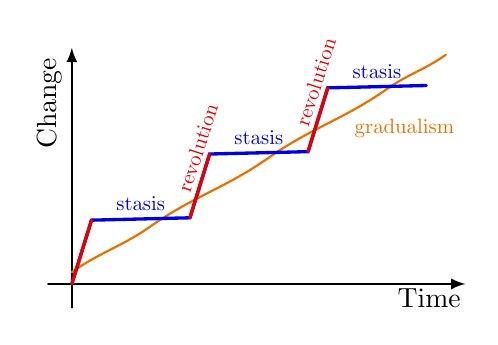
\begin{tikzpicture}[line cap=round] %[xscale=4,yscale=2]
  \def\xmax{5}
  \def\ymax{3}
  \def\xb{0.95*\xmax}
  \def\ya{0.05*\ymax}
  \def\yb{0.97*\ymax}
  \def\y#1{{\ya+(\yb-\ya)/(\xb)*#1}}
  \draw[->,thick] (-0.1*\ymax,0) -- (\xmax,0) node[below left=-2] {Time};
  \draw[->,thick] (0,-0.1*\ymax) -- (0,\ymax) node[above left,rotate=90] {Change};
  \draw[thick,myorange]
    (0,\ya)
      to[out=35,in=-145] (0.2*\xmax,\y{0.2*\xmax})
      to[out=35,in=-145] (0.5*\xmax,\y{0.5*\xmax})
      to[out=35,in=-145] (0.8*\xmax,\y{0.8*\xmax}) %node[below right,scale=0.75,myorange] {gradualism};
      to[out=35,in=-145] (\xb,\yb);
  \node[below right,scale=0.75,myorange] at (0.7*\xmax,\y{0.7*\xmax}) {gradualism};
  \draw[very thick,myblue]
    (0,0) coordinate (O) --++
    (0.05*\xmax,0.27*\ymax) coordinate (A1) --++
    (0.25*\xmax,0.01*\ymax) coordinate (A2) node[midway,above,scale=0.75] {stasis} --++
    (0.05*\xmax,0.27*\ymax) coordinate (B1) --++ %node[above,scale=0.5,rotate=60] {revolution} --++
    (0.25*\xmax,0.01*\ymax) coordinate (B2) node[midway,above,scale=0.75] {stasis} --++
    (0.05*\xmax,0.27*\ymax) coordinate (C1) --++ % node[above,scale=0.5,rotate=60] {revolution}
    (0.25*\xmax,0.01*\ymax) coordinate (C2) node[midway,above,scale=0.75] {stasis};
  \draw[very thick,myred]
    (O) -- (A1)
    (A2) node[left=3,above right=5,scale=0.75,rotate=72] {revolution} -- (B1)
    (B2) node[left=3,above right=5,scale=0.75,rotate=72] {revolution} -- (C1);
  
\end{tikzpicture}


\end{document}